
\chapter{\IfLanguageName{dutch}{Praktische uitvoering van ANPR}{Implementation of ANPR at UGent}}
\label{ch:praktischeUitvoering}
In dit hoofdstuk zal er onderzocht worden of nummerplaatdetectie degelijke resultaten kan leveren op de Campus Sterre en Campus Coupure van UGent. Hiervoor zullen handmatig foto's genomen worden van wagens die de parking willen verlaten met de Pi-NoIR cam. Hierna wordt er gecontroleerd of OpenANPR wel degelijk correcte resultaten levert op de genomen foto's.


\section{Hardware en software}
In dit onderdeel wordt de opstelling en configuratie van de camera's uitgelegd adhv. de informatie verzameld in Hoofdstuk \ref{ch:maatregelingenanpr}.

\subsection{Camera}
Als camera zal gebruik gemaakt worden van de PiNoIR-Cam. Deze camera is een standaard extensie voor de Raspberry-PI die geen infrarood filtering heeft staan. Standaard wordt infrarood uit afbeeldingen gefilterd omdat deze een ongewenst bijproduct zijn op foto's. De PiNoIR camera filtert geen infrarood uit de afbeeldingen en maken het dus mogelijk om te gebruiken voor infrarood detectie.

\paragraph{Cameraplaatsing}
Voor de plaatsing van de camera's wordt er gewenst zo veel mogelijk kosten te besparen en wordt er liever niet geopteerd voor een aparte paal voor de ANPR-camera. Daarom zal als fotopunt de metalen constructie van de hefboom gekozen worden. De camera zal hier zo hoog mogelijk aan worden gehangen zodat deze zo min mogelijk interferentie heeft van de koplampen van de auto's.

\begin{figure}[h!]
	\centering
	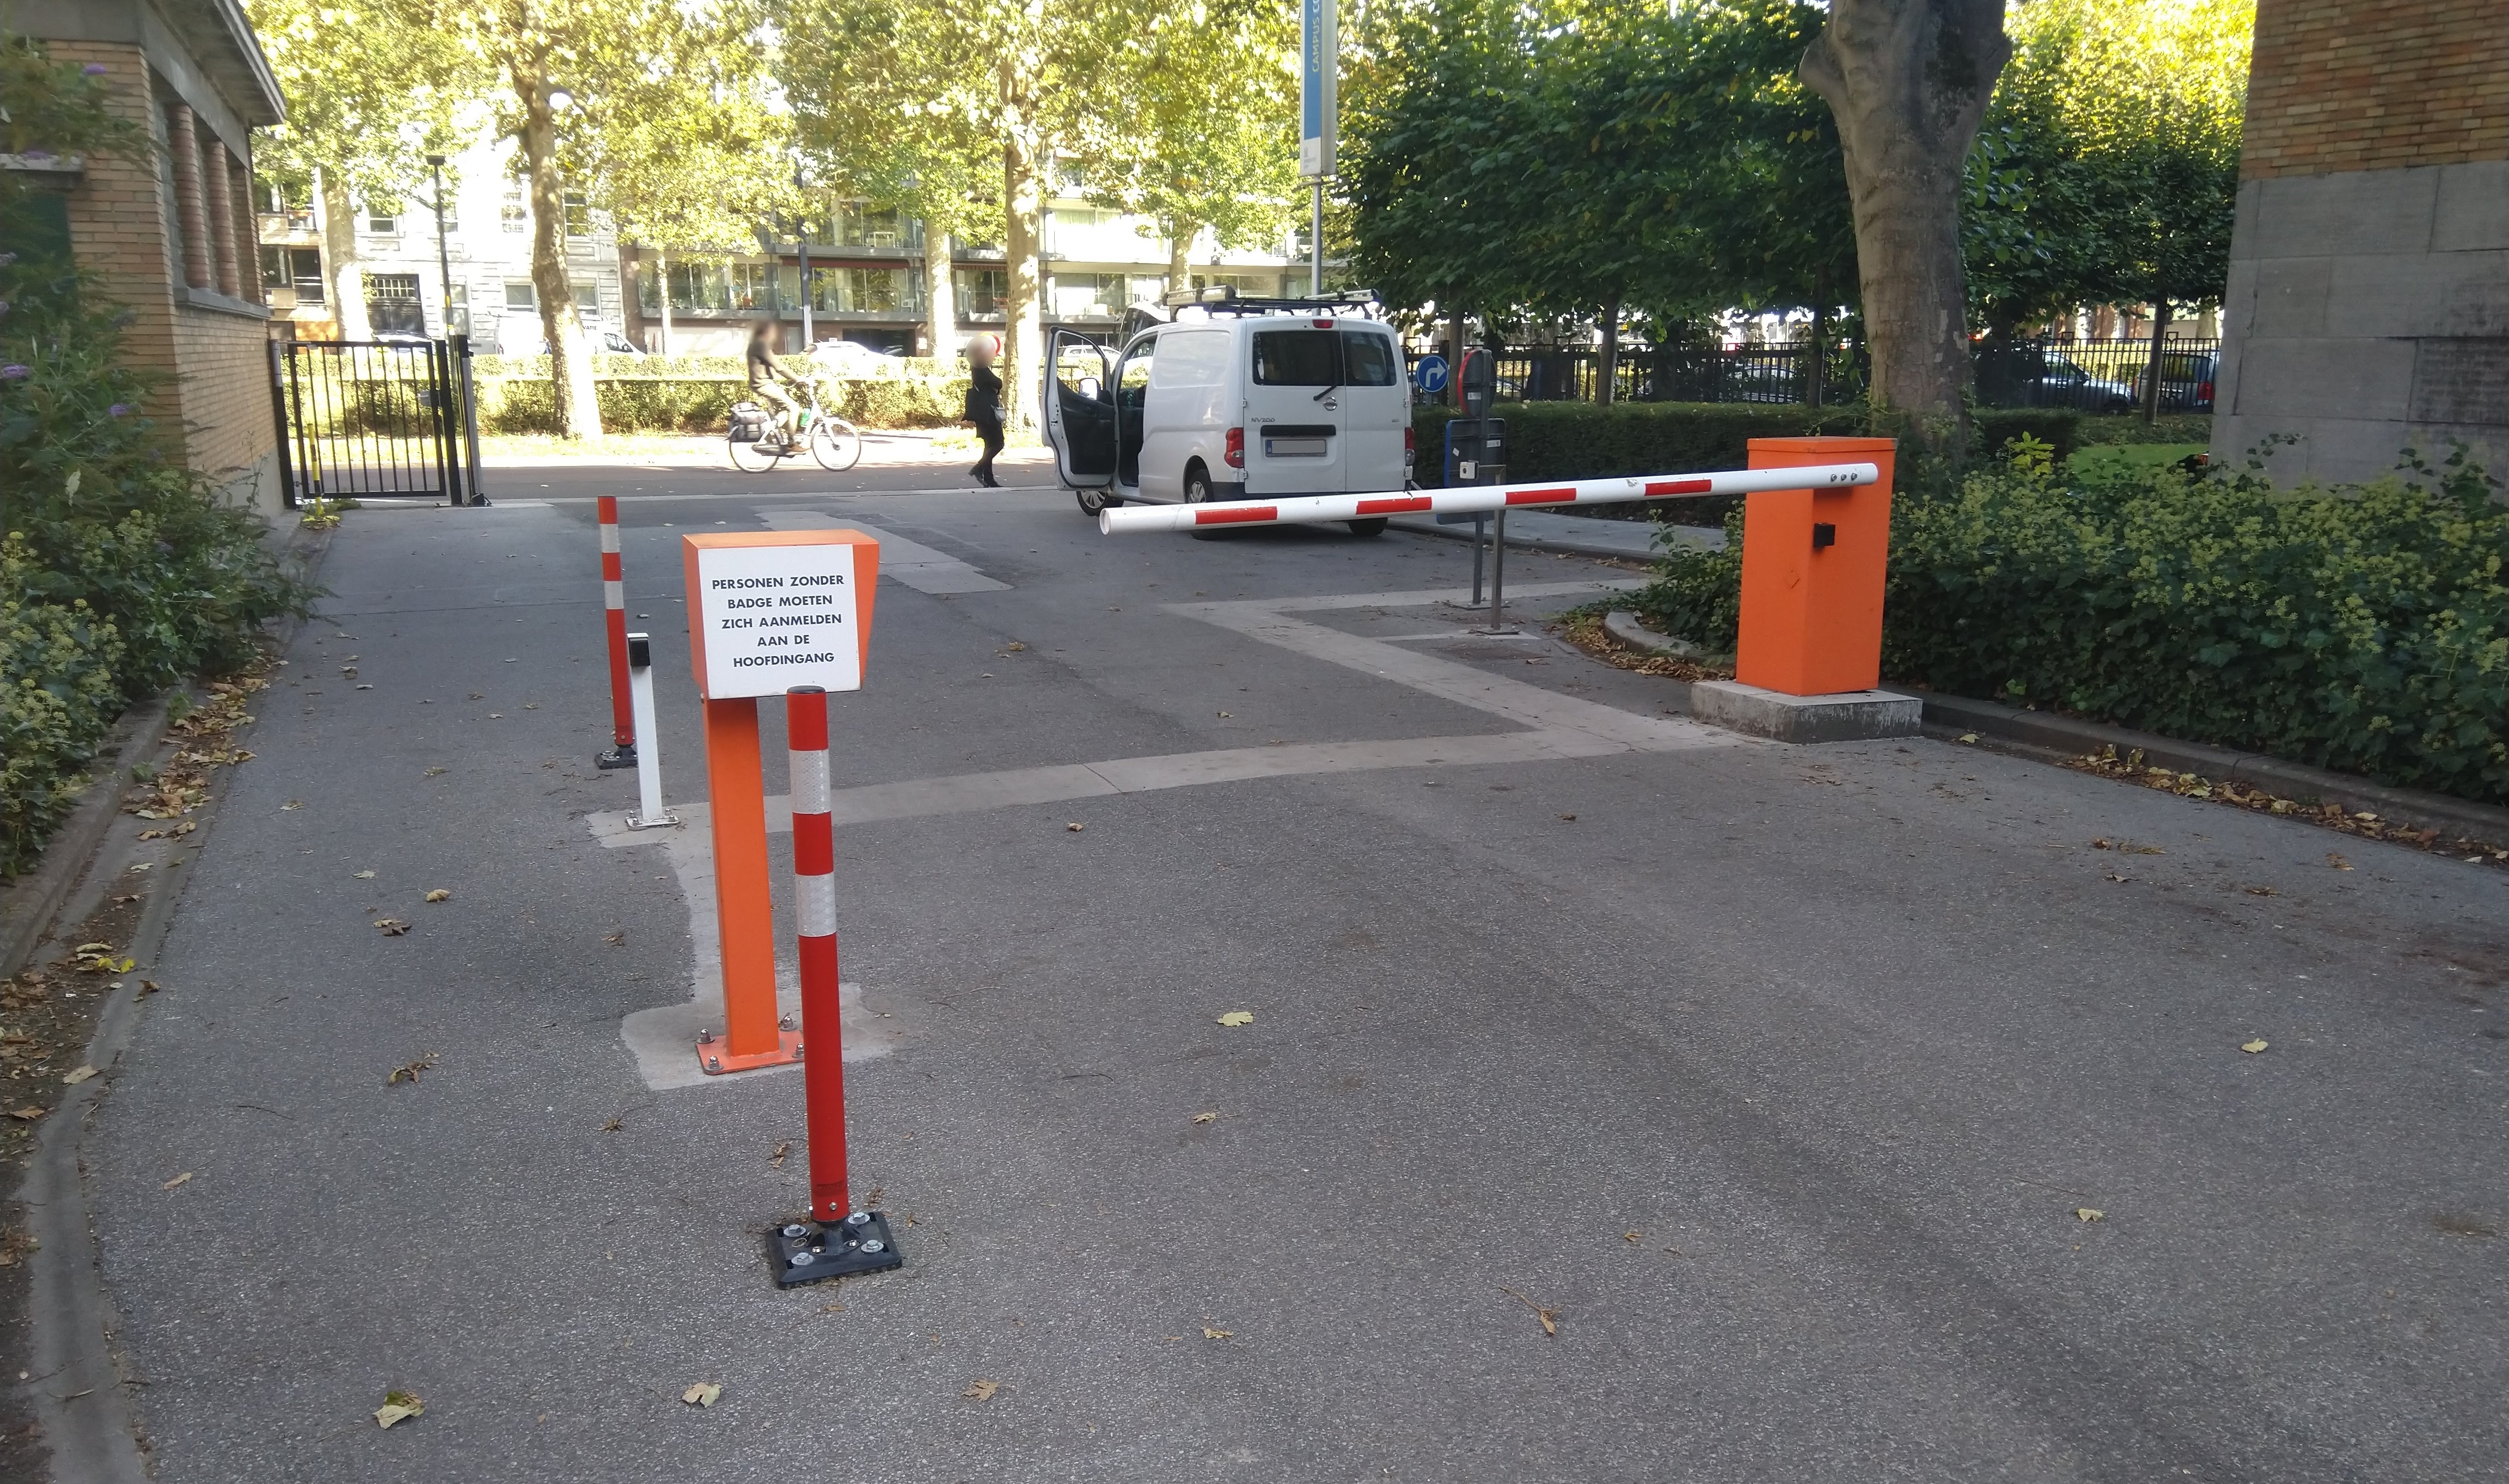
\includegraphics[width=\linewidth]{img/uitgang-coupure.jpg}
	\caption{Uitgang met tokens aan UGent campus Coupure}
\end{figure}

\paragraph{Cameraconfiguratie}
De voorgaande camerainstellingen zullen zo correct mogelijk op de PiNoIR camera worden ingesteld.
TODO: configuratie bepalen

\section{Dataset}
Om een correcte dataset te bekomen zal er op de parking van UGent zelf data verzameld worden aan de uitgangen.

Aan alle vier de uitgangen zullen in totaal een hondertal foto's genomen worden van voertuigen die de parking verlaten in verscheidene omstandigheden zoals licht/donker/regen en zal bij iedere foto genoteerd worden welke nummerplaat dit was. Zo kan er later vergeleken worden of de juiste resultaten bekomen zijn.

\subsection{Opstelling}
Om de foto's te verkrijgen zal gebruik gemaakt worden van de Raspberry Pi met de PiNoIR camera, deze zal in een behuizing op de juiste hoogte van de paal tijdelijk vastgezet worden tesamen met een powerbank. Om het signaal te sturen dat de Raspberry Pi een foto moet nemen zal deze ingesteld worden als Access Point, zo kan er via een GSM een SSH verbinding gemaakt worden waarop men de camera bestuurt.

TODO: Opstelling camera maken en fotograferen, met duct tape tijdelijk vasthangen?

\section{Verwerking van gegevens}

%Opslitsen data voor dag, nacht, regen en verschillende ingangen/uitgangen.
%alpr uitvoeren op alle afbeeldingen en checken of ze correct zijn. Rekening houden met orientatie zodat de publieke weg niet in beeld is.